The \ref{fig:component_diagram} represents the Safestreets component diagram. Each of the components are wrapped inside a specific box that indicates the subsystem in which they belong to.
\newline Subsystems are groups of components which perform similar operations: this boxing technique is a multilayer logical division that can be useful in order to categorize the components and the whole system at different layers of abstraction.
\newline For the sake of simplicity, the component diagram pictures the application layer (backend) of the system and not the mobile and web app structures. The business logic and core functions are fully contained in the application layer and therefore only that relevant part of the Safestreets system has been characterized.
\begin{figure}[H]
    \centering
    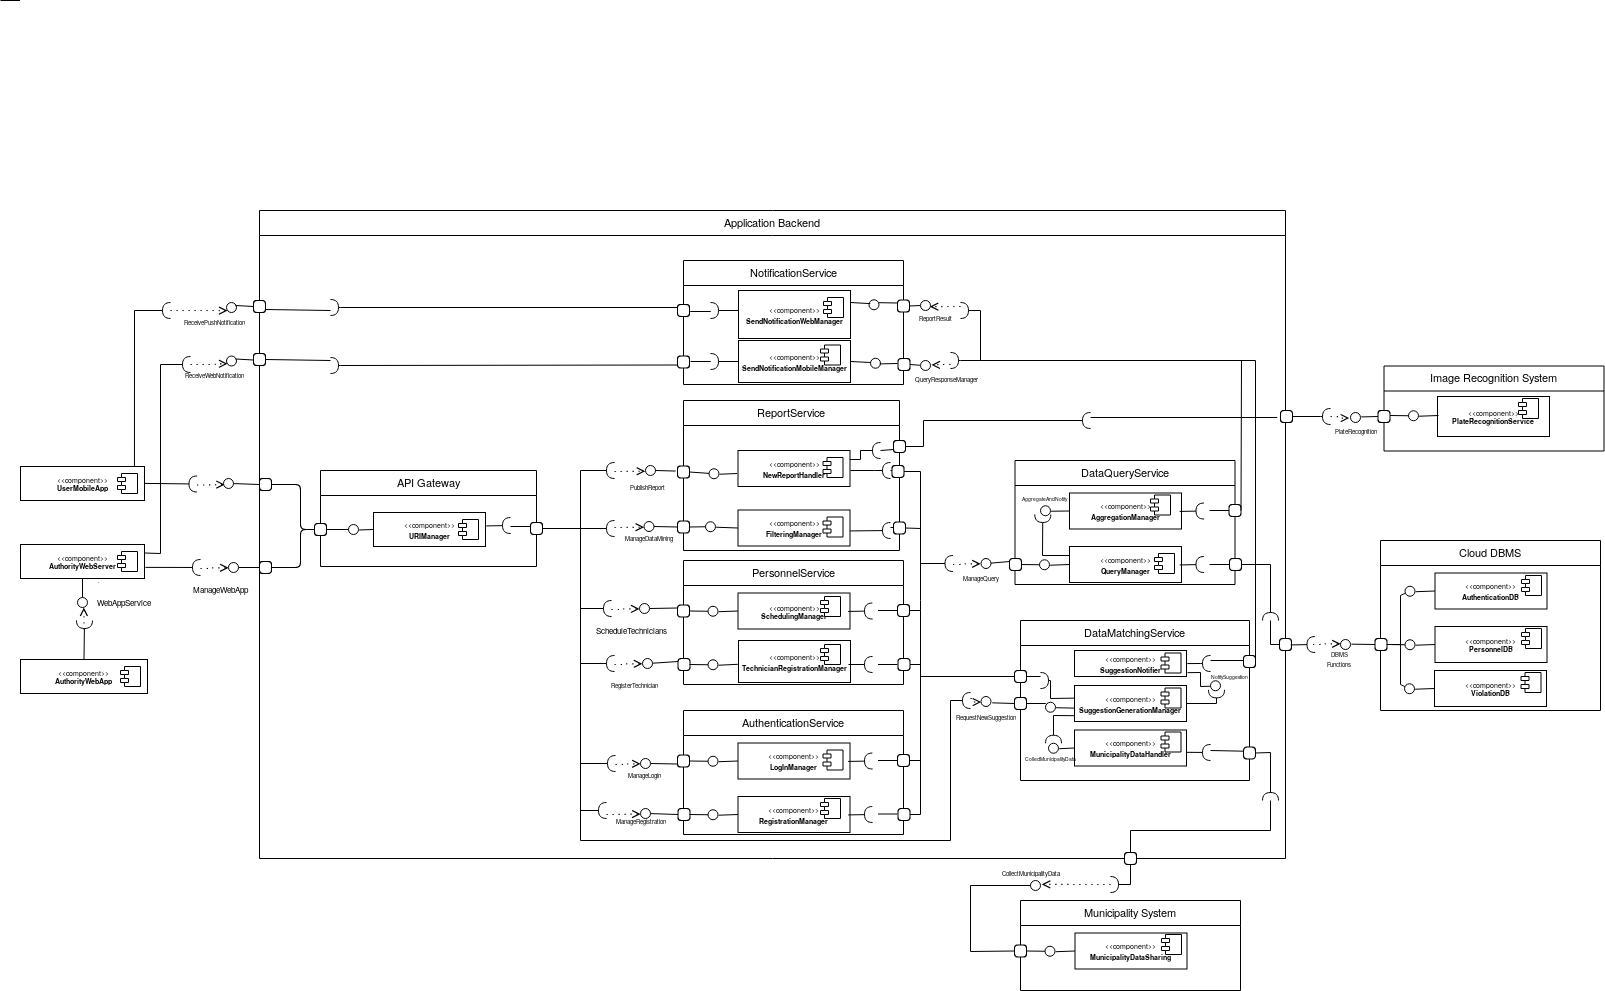
\includegraphics[width=1.1\textwidth]{UML_diagrams/component_uml_safestreets}
    \caption{Component UML diagram}
    \label{fig:component_diagram}
\end{figure}
Here it is a detailed explanation for each of the components shown in the component diagram:
\begin{itemize}
    \item 
    \item 
    \item 
    \item 
    \item 
    \item 
    \item 
    \item 
    \item 
    \item 
    \item 
    \item 
    \item 
    \item 
    \item 
    \item 
    \item 
    \item 
    \item 
    \item 
    \item 
    \item 
    \item 
\end{itemize}